% Author: Dr. Matthias Jung, DL9MJ
% Year: 2020
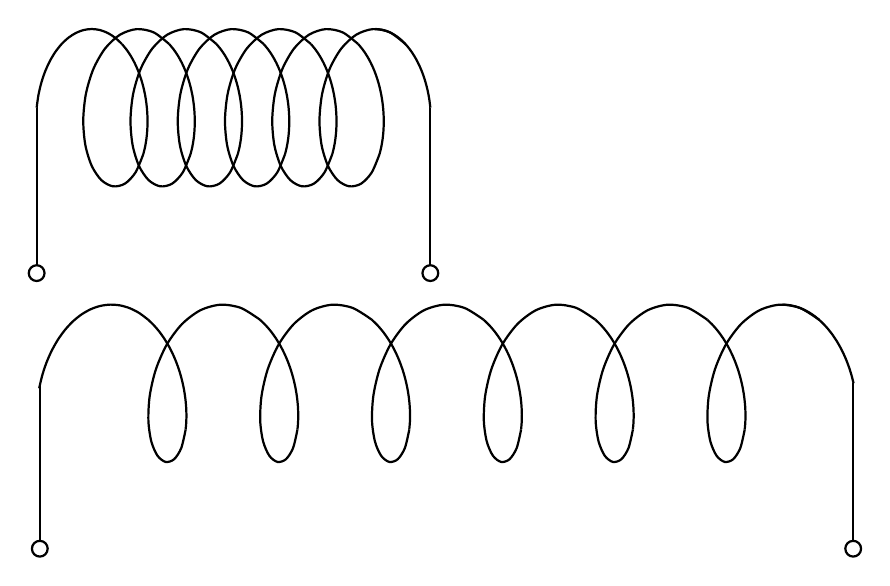
\begin{tikzpicture}
    % Define a formula for the coil.
    % This is what the numbers mean:
    % A ... how far the rings are apart
    % B ... how much from the side the rings are seen (try 0 and the same as the radius)
    % C ... radius of the rings
    \def\coil#1{
        % A                   B
        {0.3 * (2*#1 + \t) + 0.55*sin(\t * pi r))},
        % C
        {1.0 * cos(\t * pi r)}
    }

    % Draw the part of the coil behind the rectangle
    \foreach \n in {0,1,...,5} {
        \draw[domain={0.2:0.7},smooth,variable=\t,samples=15, thick]
            plot (\coil{\n}); 
        }

    % Draw the part of the coil in front of the rectangle
    \foreach \n in {0,1,...,5} {
        \draw[domain={0.7:2.2},smooth,variable=\t,samples=15, thick]
            plot (\coil{\n});
        }

    \draw[domain={ 0.0:0.5},smooth,variable=\t,samples=15,thick] plot (\coil{6});
    \draw[domain={-0.5:0.2},smooth,variable=\t,samples=15,thick] plot (\coil{0});
    \draw[thick](-0.7,0) -- (-0.7,-2);
    \draw[thick](4.3,0) -- (4.3,-2);
    \draw[thick](4.3,-2.1) circle (0.1);
    \draw[thick](-0.7,-2.1) circle (0.1);

\begin{scope}[yshift=-3.5cm, xshift=0.25cm]

    % Define a formula for the coil.
    % This is what the numbers mean:
    % A ... how far the rings are apart
    % B ... how much from the side the rings are seen (try 0 and the same as the radius)
    % C ... radius of the rings
    \def\coil#1{
        % A                   B
        {0.710 * (2*#1 + \t) + 0.55*sin(\t * pi r))},
        % C
        {1.0 * cos(\t * pi r)}
    }

    % Draw the part of the coil behind the rectangle
    \foreach \n in {0,1,...,5} {
        \draw[domain={0.2:0.7},smooth,variable=\t,samples=15, thick]
            plot (\coil{\n}); 
        }

    % Draw the part of the coil in front of the rectangle
    \foreach \n in {0,1,...,5} {
        \draw[domain={0.7:2.2},smooth,variable=\t,samples=15, thick]
            plot (\coil{\n});
        }

    \draw[domain={ 0.0:0.5},smooth,variable=\t,samples=15,thick] plot (\coil{6});
    \draw[domain={-0.52:0.2},smooth,variable=\t,samples=15,thick] plot (\coil{-0.0});
    \draw[thick](-0.91,0) -- (-0.91,-2);
    \draw[thick](9.42,0) -- (9.42,-2);
    \draw[thick](9.42,-2.1) circle (0.1);
    \draw[thick](-0.91,-2.1) circle (0.1);
\end{scope}
\end{tikzpicture}